\section{Discussion and Conclusion}\label{sec:conclusion}

We have measured the local PNG parameter $\fnl$ using the scale-dependent bias in the angular clustering of LRGs selected from the DESI Legacy Imaging Survey DR9. Our sample includes more than $12$ million LRG targets covering around $14,000$ square degrees in the redshift range of $0.2< z < 1.35$. We leverage early spectroscopy during DESI Survey Validation \citep{desi2023sv} to infer the redshift distribution of our sample (Figure \ref{fig:nz}). \mr{Our power spectrum model accounts for various theoretical and observational effects such as RSD, magnification bias, survey geometry, and integral constraint. Most importantly, we utilize a novel machine learning-method to mitigate the effect of imaging systematics and reduce excess clustering power at low $\ell$.} In our fiducial analysis, \mr{which includes non-linear treatment using three maps (extinction, depth in z, and psfsize in r),} we have obtained a maximum likelihood value of \mr{$\fnl=46$} with a significant probability that $\fnl$ is greater than zero, $P(\fnl>0)=99.9$ (Figure \ref{fig:mcmc_dr9} and Table \ref{tab:dr9methodcalib}).

The signature of local PNG is very sensitive to excess clustering signals caused by imaging systematic effects. We have applied a series of robustness tests to investigate the impact of how the galaxy selection function is determined. Specifically, both linear and nonlinear methods are applied using various combinations of imaging systematic maps (Galactic extinction, stellar density, depth in $grzW1$, psfsize in $grz$, and neutral hydrogen column density). We also examine the effect of different masks based on imaging. Overall, we find no change in the analysis that shifts the maximum likelihood value of $\fnl$ to a significantly lower value (Figure \ref{fig:mcmc_dr9reg}, Figure \ref{fig:mcmc_dr9elmin}, and Table \ref{tab:dr9method}). The only manner in which the significance of nonzero PNG decreases is due to the uncertainty on the measurement increasing when we employ more imaging systematic maps for the selection function estimation and by doing so remove large-scale clustering information (the effect of which on $\fnl$ recovery we have calibrated with mocks, as shown in Figure \ref{fig:fnlbias}). \mr{For instance, we obtain $\fnl = 34^{+24(+50)}_{-44(-73)}$ using the nonlinear nine maps method.}

\begin{figure}
    \centering
    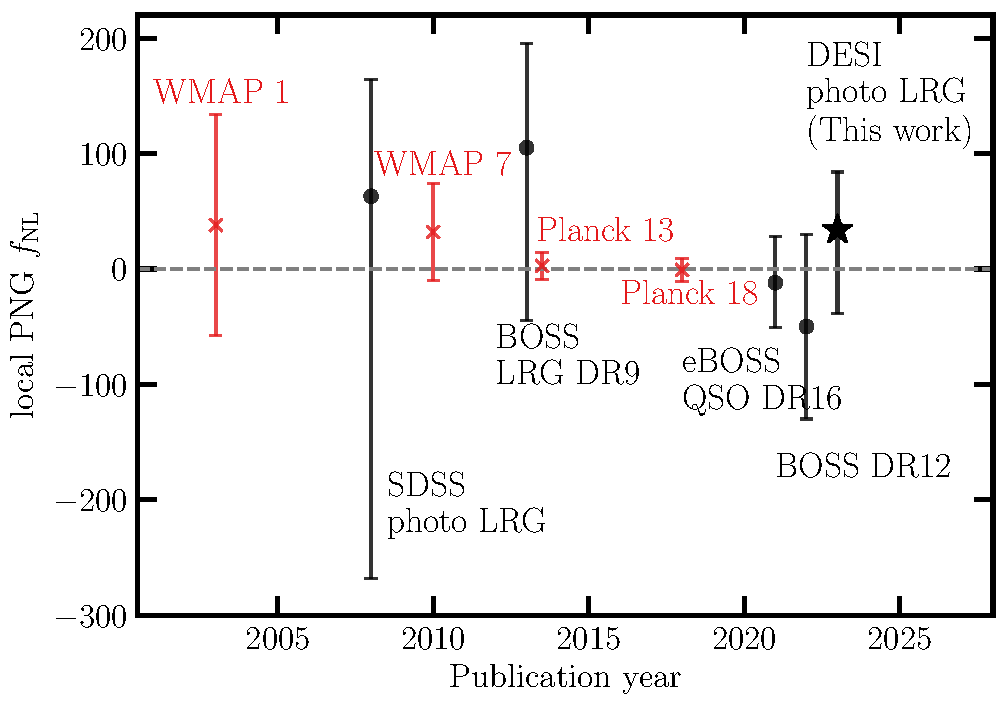
\includegraphics[width=0.45\textwidth]{figures/fnl_history.pdf}
    \caption{History of constraints on local PNG $\fnl$ at $95\%$ confidence from single-tracer LSS \citep{slosar2008constraints,2013MNRAS.428.1116R, mueller2022primordial, 2022PhRvD.106d3506C}, including our analysis with $\mr{21}<\fnl<76$ (DESI photo LRG) and CMB surveys \citep{Komatsu_2003, Komatsu_2010, planck13, akrami2019planck}. The median $\fnl$ value is used in case the maximum likelihood estimate was not reported in the reference.}
    \label{fig:fnlhist}
\end{figure}

When comparing our fiducial results to recent CMB and QSO measurements, as shown in Figure \ref{fig:fnlhist}, we find a significant tension with CMB\mr{, e.g., more than $3 \sigma$ at $p=1$ (see Figure \ref{fig:fnl_magbias}),} but consistent constraints with LSS within $95\%$ confidence. \mr{Our findings are robust against parameters $p$ and $s$. The tension between our non-linear three maps constraint and CMB is significant even without accounting for over-correction with $P(\fnl>0)=99.5$ per cent. The linear methods also yield constraints that are in tension with CMB ($P(\fnl>0)=99.9$), and while we have not calibrated the over-correction for the linear cases, it would only make the result more significantly non-zero and we cannot envision this changing any of our conclusions. The only approaches that return constraints consistent with CMB are the ones that diminish the constraining power of the dataset, such as non-linear nine maps. Given our mean density and cross power spectrum $\chi^{2}$ tests (Appendix \ref{sec:systests}), when compared to the mocks with $\fnl=0$, non-linear three maps provides sufficient cleaning for systematics that we have the imaging maps for.} Therefore, either we have measured an $\fnl$ signal that is inconsistent with CMB measurements or there is a hidden source of systematic contamination in our data which cannot be mitigated with available imaging systematic maps. \mr{Cross-correlations of the DESI LRG density with the CMB lensing map can shed more light on the source of the excess power measured in this work. In future work, we aim at improving the estimation of the galaxy survey selection function by combining our neural network method with forward-modeling techniques, such as Obiwon \citep{kong2020}.}

Our analysis can be considered as the first attempt to identify major systematics in DESI, so we can be ready for constraining $\fnl$ with DESI spectroscopy. Internal DESI tests of the photometric calibration were unable to uncover DESI-specific issues, e.g., when comparing to Gaia data. The most significant trends that we find are with the E(B-V) map. The source of such a trend would be a mis-calibration of the E(B-V) map itself or the coefficients applied to obtain Galactic extinction corrected photometry. Such a mis-calibration would plausibly be proportional in amplitude to the estimated E(B-V) map, though it may not have E(B-V)’s spatial distribution. In order to explain the $\fnl$ signal we measure, such an effect would need to be approximately twice that of the trend we find with E(B-V). There are ongoing efforts within DESI to obtain improved Galactic extinction information, which will help establish if this is indeed the cause.

\mr{There is a body of exciting work in the literature exploring models where $\fnl$ (or another non-Gaussianity parameter) varies with scales and evades the CMB constraint while showing up in the LSS \citep{2008JCAP...04..014L,sefusatti_2009, becker_2011, Becker_2012}. For instance, \cite{Becker_2012} presents forecasts on $\fnl(k)$ from the Planck bispectrum and DES power spectrum assuming the power-law model of scale-dependent non-Gaussianity, and illustrate the difference in the optimal wavenumber for CMB and LSS probes. Thus, in principle, CMB and LSS can measure different $\fnl$ values, but whether and what kind of specific scale dependent $\fnl$ model would be consistent with our measurement and the CMB measurement would require detailed work.}